\documentclass[e4_tp1_main.tex]{subfiles}

\begin{document}

\section{Ejercicio 1}
Se procederá al análisis del circuito de la \autoref{fig:circuit_1}. El mismo es un circuito destinado al análisis del disparo de un transistor MOSFET.


\begin{figure}[H]
  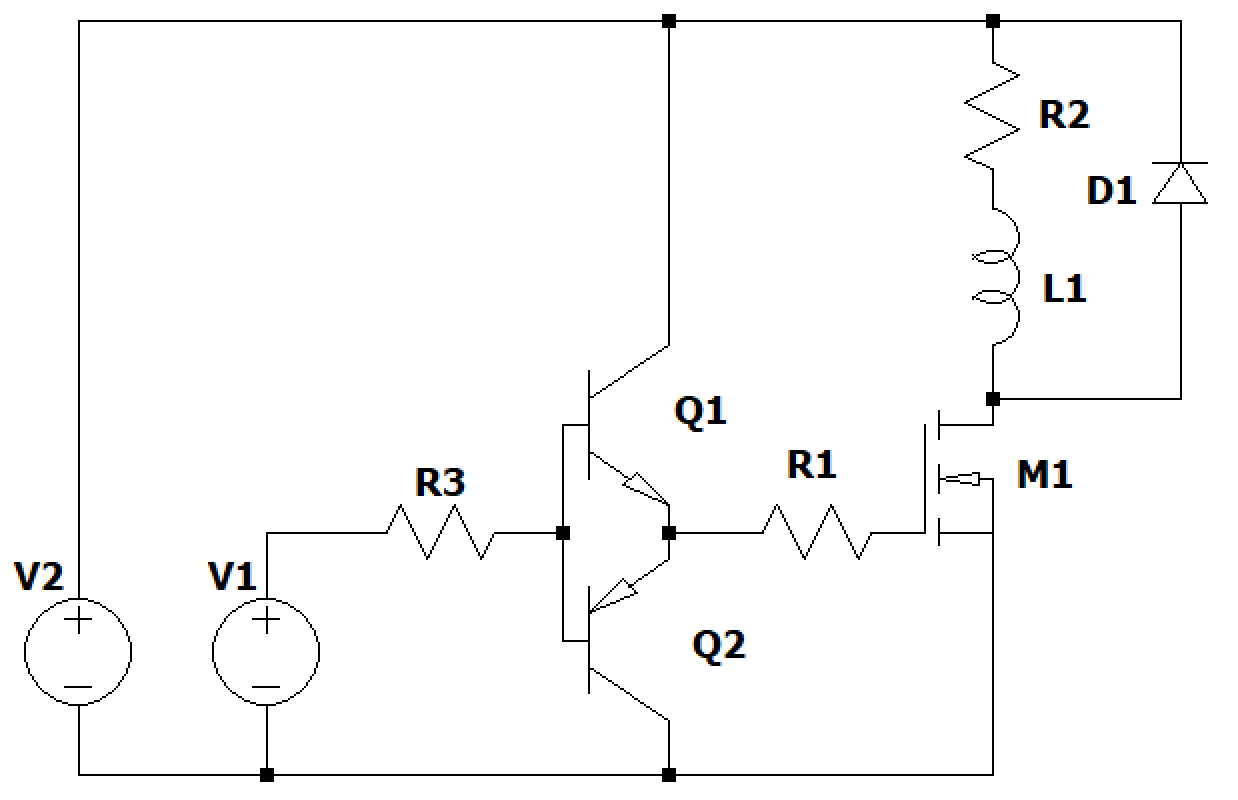
\includegraphics[width=\linewidth]{images/ej1/circuit_1.png}
  \caption{Circuito para análisis de disparo de transistor MOSFET}
  \label{fig:circuit_1}
\end{figure}

\subsection{Circuito Driver}

Los transistores $Q_1$ y $Q_2$ forman una configuración Totem-Pole, y se encuentran funcionando en saturación (push-pull output). 
Nótese que para prender el transistor, se requiere cargar las capacidades internas del MOSFET, por lo que se requiere un pico de corriente que un generador de señales no es capaz de proveer. Utilizando esta configuración, se puede activar y desactivar este circuito utilizando un generador de señales, mientras que la corriente es provista por la fuente de tensión.
Idealmente, la salida de este circuito valdrá $V_{out} = V_1 - 0.7V$ cuando el circuito esté activado, y $V_{out} = 0.7V$ cuando se encuentre desactivado. Este circuito afectará la curva de control del Gate, pues la misma no es un escalón ideal. Se tendrá en cuenta el delay para la interpretación de los resultados obtenidos, pero no nos centraremos en el análisis de los delays de esta configuración.

\subsection{Conmutación MOSFET}

Durante la conmutación del MOSFET, circula corriente por el Gate. Esta corriente es debido a capacidades internas del transistor, que se cargan durante la conmutación. Dichas capacidades corresponden básicamente a las cargas de la capa de inversión e ionización que se forman en el body del transistor para formar el canal N (Capacidad Gate-Source $C_{GS}$ - recordar que el Gate y el Source se encuentran cortocircuitados internamente), y las cargas asociadas a la capa de acumulación o de deplexión que se forma en el Drain del transistor (Capacidad Gate-Drain $C_{GS}$), que ayudan a minimizar la resistencia del MOSFET cuando se encuentra activado. Cabe destacar que estas capacidades dependen del tamaño de la capa de acumulación / deplexión, y por lo tanto cambian durante la conmutación del MOSFET. Se buscará introducir las ecuaciones a utilizar, sin entrar en detalle sobre el funcionamiento del transistor.

\subsubsection{Encendido del MOSFET}

Considerando que, ante un escalón de tensión en provisto por el circuito Driver, dichas capacidades comienzan a cargarse, se puede modelar la primera etapa del prendido del MOSFET con un circuito RC, por lo que la tensión $V_{G}$ en función del tiempo puede ser aproximada por
\begin{equation}
V_G(t) = V_1 (1-\exp(-t/\tau_1)).
\end{equation}
donde $\tau_1 = R_1\tilde{C}_{G,1}$ y $\tilde{C}_{G,1} = C_{GS} + C_{GD,1}$. Cuando la tensión en el Gate llega a $V_{GS,th}$ (en $t=t_{d,on}$), comienza a formarse la capa de inversión, por lo que la corriente del drain $I_D$ comienza a aumentar hasta llegar al valor $I_0$ impuesto por la carga inductiva y que el diodo deje de conducir (en $t=t_1$). Esto ocurrirá cuando la tensión en el Gate llegue a un valor $V_G=V_{G,I_D=I_0}$. El tiempo entre que comienza a circular corriente hasta que se alcanza el valor $I_0$ se denomina $t_{ri}$. Se puede demostrar que

\begin{equation}
t_{d,on} = -\tau_1 \ln\left(1-\frac{V_{G,th}}{V_1}\right)
\end{equation}
\begin{equation}
t_{1} = -\tau_1 \ln\left(1-\frac{V_{G,I_D=I_0}}{V_1}\right)
\end{equation}
\begin{equation}
t_{ri} = t_{1} - t_{d,on}.
\end{equation}

Luego, cuando la corriente de drain llega al valor $I_0$, el valor de la tensión en el gate se mantiene temporalmente en $V_G=V_{G,I_D=I_0}$, por lo que la capacidad $C_{GS}$ deja de cargarse, mientras se sigue cargando $C_{GD}$ a corriente constante. A medida se cargue $C_{GD}$ se formará la capa de acumulación, bajando la resistencia $R_{DS}$, por lo que disminuye la tensión $V_{DS}$ hasta alcanzar el valor $V_{DS,on}$. Dado que la capacidad $C_{GD}$ varía durante este proceso, pues varían la longitud de la capa de acumulación, suele utilizarse el valor de la carga total $\Delta Q$ para estimar la duración de esta etapa. Con esto, el tiempo que transcurre desde que empieza a caer la tensión $V_{DS}$ hasta que alcanza el valor$V_{DS,on}$ puede estimarse según:

\begin{equation}
t_{fv} = \Delta Q/I_{G,on} = \frac{\Delta Q R_1}{V_{1}-V_{G,I_D=I_0}}
\end{equation}

A lo largo de esta etapa, cambia el valor de $C_{GD,1}$ a $C_{GD,2}$. Luego, la tensión en el Gate sigue creciendo hasta llegar al valor $V_{GG}$. El tiempo característico asociado está dado por:

\begin{equation}
\tau_2 = R_1\tilde{C}_{G,2}
\end{equation}
Donde $\tilde{C}_{G,2} = C_{GS} + C_{GD,2}$

\subsubsection{Apagado del MOSFET}

El apagado del MOSFET es similar al encendido, pero en orden contrario:

Primero, se comienzan a descargar las capacidades internas por el Gate, por lo que la tensión del Gate en la primera etapa está dada por:

\begin{equation}
V_G(t) = V_{GG} \exp(-t/\tau_2)
\end{equation}

Esto ocurrirá hasta que la tensión $V_G$ alcance el valor $V_{G,I_D=I_0}$ en $t=t_2$. Puede demostrarse que:
\begin{equation}
t_2= -\tau_2\ln\left(\frac{V_{G,I_D=I_0}}{V_{GG}}\right)
\end{equation}

Luego, la tensión en el Gate permanecerá constante mientras se descarga $C_{GD,2}$ a corriente constante durante un tiempo $t_{rv}$. Analogo al caso de encendido, este tiempo está dado por
\begin{equation}
t_{rv} = \Delta Q/I_{G,off} = \frac{\Delta Q R_1}{V_{G,I_D=I_0}}
\end{equation}

Notar que, al igual que durante el prendido, la capacidad $C_{GD}$ cambia de valor durante este proceso. Finalmente, la tensión en el Gate baja según la ecuación
\begin{equation}
V_{G} = V_{G,I_D=I_0}\exp(-t/\tau_1).
\end{equation}

A medida que la tensión cae, comienza a deshacerse el canal formado, por lo que baja el valor de $I_D$ hasta hacerse nulo cuando $V_G=V_{G,th}$. Esto ocurre luego de un intervalo $t_{fi}$. El valor de $t_{fi}$ está dado por
\begin{equation}
t_{fi}= -\tau_1\ln\left(\frac{V_{G,th}}{V_{G,I_D=I_0}}\right).
\end{equation}

Un gráfico esquemático mostrando la conmutación del MOSFET se muestra en la \autoref{fig:mosfet_theory}


\begin{figure}[H]
  \centering
  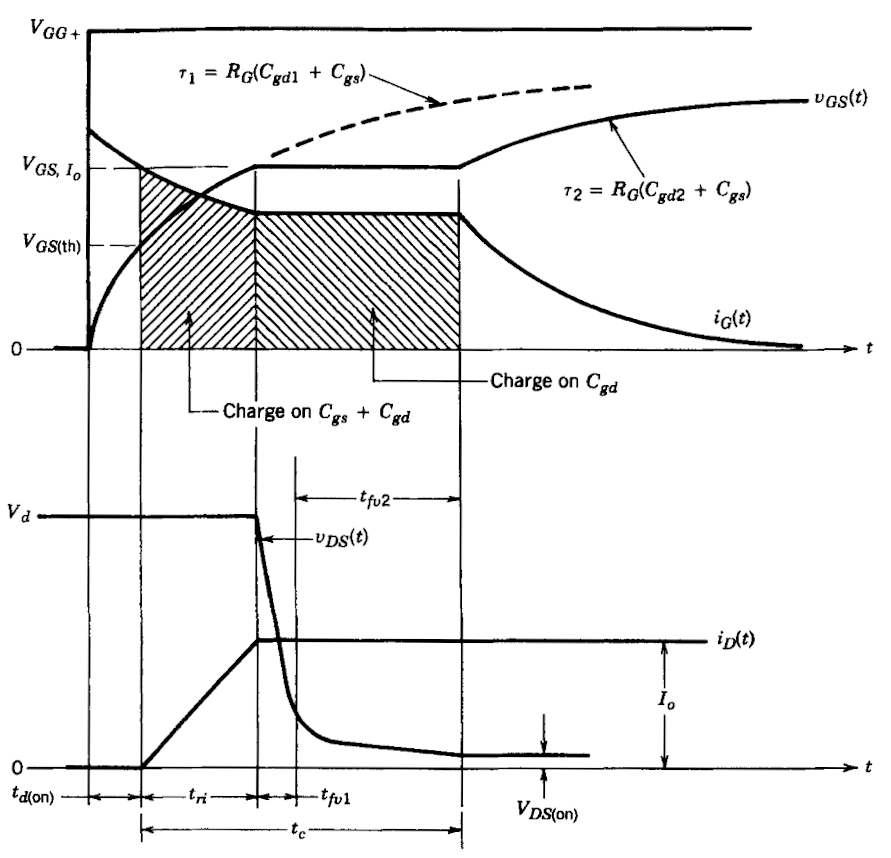
\includegraphics[width=\linewidth/2]{images/ej1/theory_mosfet.png}
  \caption{Curvas de tensión y corriente en el MOSFET durante el encendido}
  \label{fig:mosfet_theory}
\end{figure}


\subsection{Carga Inductiva}
La carga está compuesta por un circuito RL. Los valores importantes a tener en cuenta para el análisis del circuito son la corriente nominal y su tiempo característico. La corriente nominal se obtiene considerando que el MOSFET se comporta como una llave cerrada. El valor de la corriente está dado por
\begin{equation}
I_0 = V_2/R_2.
\end{equation}
El tiempo característico de este circuito está dado por
\begin{equation}
\tau_{RL} = L_1/R_2.
\end{equation}

\subsection{Diodo}
También resulta importante analizar la dinámica del Diodo durante la conmutación, dado que afecta a las curvas de conmutación del MOSFET, que es lo que se busca analizar en este punto. Con este objetivo, se realizará un breve análisis de la conmutación de un diodo real. El análisis se realiza considerndo un switch que impone un cambio de corriente $di/dt$. Recordar que un diodo de potencia está formado por dos junturas: $p^+n^-n^+$.

\begin{figure}[H]
  \centering
  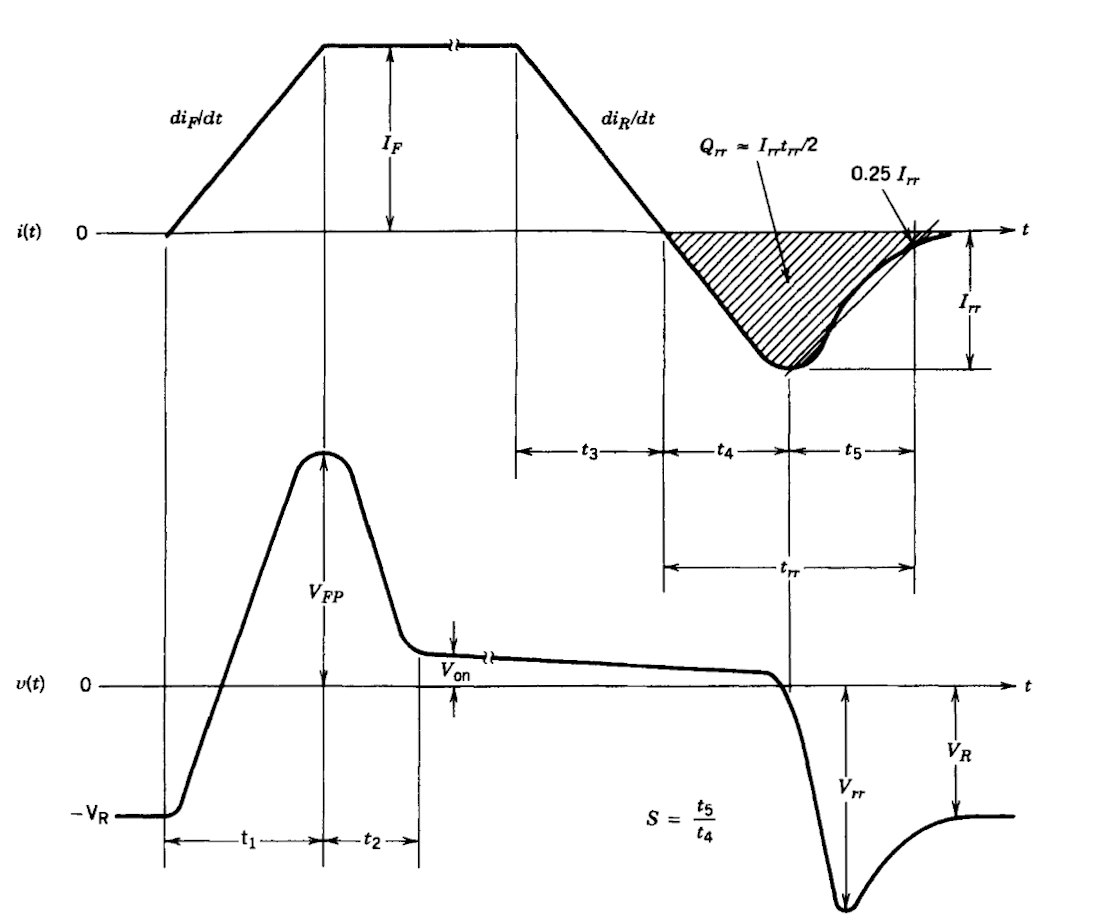
\includegraphics[width=\linewidth/2]{images/ej1/diode.png}
  \caption{Curvas de encendido y de apagado de un diodo de potencia (tensión y corriente)}
  \label{fig:diode}
\end{figure}

\subsubsection{Encendido del Diodo}
Cuando el diodo se encuentra polarizado en inversa y se lo prende, la corriente sube de acuerdo al $di/dt$ impuesto por el circuito, a medida que se restaura la carga en la zona de deplexión hasta el valor de equilibrio térmico y se comienza a polarizar en directa. A medida que el diodo se polariza en directa, baja la resistencia de este hasta que la tensión en el diodo llega a $V_{on}$. Por la corriente que circuila mientras que el diodo no está completamente polarizado y su resistencia interna es alta, se produce un pico de tensión en el diodo. Este pico puede resultar mayor considerando las inductancias parásitas, si se aplican valores altos de $di/dt$. Este overshoot puede afectar seriamente algunos circuitos de potencia. La curva de encendido del diodo se puede encontrar en la \autoref{fig:diode}.

\subsubsection{Apagado del Diodo}
El apagado del diodo es escencialmente el proceso inverso al encendido. Primero los portadores de carga libres deben ser removidos para que la juntura llegue al equilibrio térmico antes de que la misma pueda ser polarizada en inversa. Siempre que haya exceso de portadores de carga libre en las zonas de drift, las junturas estan polarizadas en directa, por lo que la tensión en el diodo no varia más alla de pequeñas diferencias por pérdidas ohmicas. Una vez que suficientes portadores de carga son removidos y la corriente se vuelve negativa, la o las junturas se polarizan en inversa, momento en el que la corriente deja de volverse más negativa y tiende al valor de cero. Este pico de corriente negativo se denomina $I_{rr}$. Durante este último intervalo hay pérdidas de potencia debido a que crece la resistencia del diodo al polarizarse en inversa, por lo que hay un pico de tensión negativo, y luego la corriente tiende a cero (y la tensión baja en módulo y tiende al valor de tensión aplicado en el diodo). La curva de apagado del diodo se puede encontrar en la \autoref{fig:diode}.

\subsubsection{Efecto de $I_{rr}$ en la conmutación del MOSFET}

El valor de $I_rr$ afecta en la conmutación del MOSFET. Nótese que este efecto se da cuando el diodo se apaga, es decir, durante el encendido del MOSFET.

Por causa de la corriente $I_rr$, la corriente de drain $I_D$ crece hasta el valor $I_0+I_rr$, por lo que el valor de $V_{G}$ crece por arriba de $V_{G,I_D=I_0}$. Cuando el diodo se recupera y la corriente vuelve a cero (y, por lo tanto, la corriente $I_D$ baja a $I_0$), el valor de $V_G$ baja a $V_{G,I_D=I_0}$, y el cambio de tensión provee corriente adicional a la capacidad $C_{GD}$, produciendo que $V_{GD}$ y $V{DS}$ decrezcan rapidamente durante este intervalo de recovery. Los efectos de la corriente $I_{rr}$ en la conmutación del MOSFET pueden observarse en la \autoref{fig:mosfer_irr}

\begin{figure}[H]
  \centering
  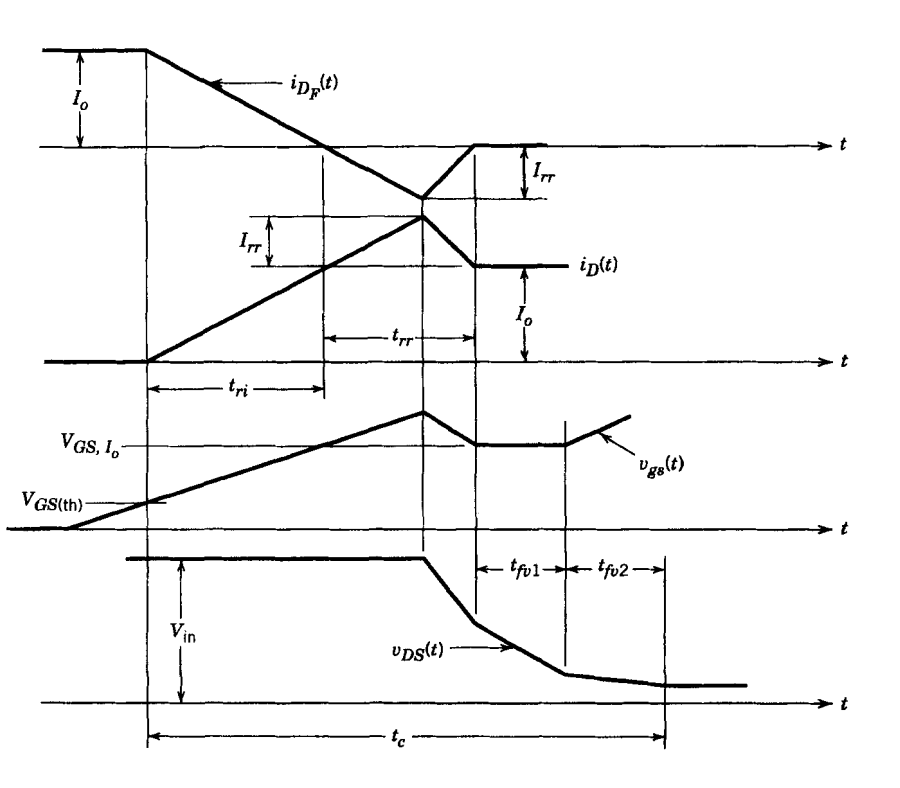
\includegraphics[width=\linewidth/2]{images/ej1/diode_irr.png}
  \caption{Efectos de $I_{rr}$ en el encendido del MOSFET.}
  \label{fig:diode}
\end{figure}

\subsection{Valores de los componentes y variables}
\begin{table}[H]
\begin{tabular}{|c|c|c|c|c|c|c|c|c|c|c|}
\hline
Componente & $Q_1$ & $Q_2$ & $R_1$ & $R_2$ & $R_3$ & $M_1$ & $L_1$ & $D_1$ & $V_2$ & $V_1$\\
\hline
Valor & BC337-25 & BC557B & 100 $\Omega$ & 15 $\Omega$ & 1 $K\Omega$ & IRF530 & 220 $\mu H$ & MUR460 & 50 V & Vp=15 V\\
\hline
\end{tabular}
\caption{Componentes}
\end{table}
Reemplazando los valores de estos, obtenemos lo siguiente:\\
\begin{tabular}{|c|c|c|c|c|c|c|c|}
\hline
Variable & $I_O$ & $V_{ds,max}$ & $V_{G,th}$ & $V_{G,I_D=I_0}$ & $\tilde{C}_{G,1}$ & $\tilde{C}_{GD,2}$ & $\Delta Q$  \\
\hline
Valor & $\frac{10}{3}$ A & 50 V & 4 V & 5,2 V & 800 pF & 650 pF & 6,25 nC\\
\hline
\end{tabular}\\
Y los tiempos de conmutación son:\\
\begin{tabular}{|c|c|c|c|c|c|c|c|}
\hline
Variable & $t_{d,on}$ & $t_{ri}$ & $t_{fv}$ & $t_{rv}$ & $t_{fi}$  \\
\hline
Valor & 24,8124 nseg A & 9,2410 nseg & 63,7755 nseg & 120,1923 nseg & 20,9891 nseg\\
\hline
\end{tabular}

Finalmente, se obtienen las siguientes curvas:
\end{document}
